\usetikzlibrary{arrows.meta,calc}
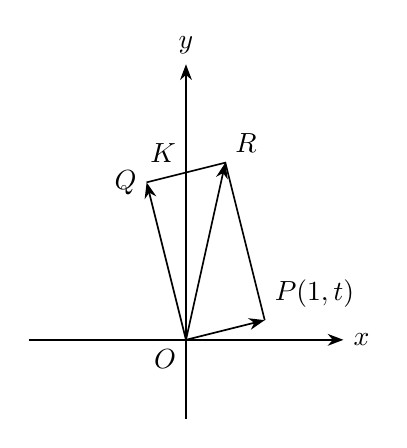
\begin{tikzpicture}[x=1cm,y=1cm,line width=.6pt,font=\normalsize,>=Stealth]
\coordinate (O) at (0,0);
\coordinate (P) at (1,0.25);
\coordinate (Q) at (-0.5,2);
\coordinate (R) at (0.5,2.25);
\coordinate (K) at (0,2.125);
\draw[->] (-2,0)--(2,0) node[right] {$x$};
\draw[->] (0,-1)--(0,3.5) node[above] {$y$};
\draw[->] (O)--(P);
\draw[->] (O)--(Q);
\draw (P)--(R)--(Q);
\draw[->] (O)--(R);
\node[below left] at (O) {$O$};
\node[above right,yshift=1pt] at (P) {$P(1,t)$};
\node[left] at (Q) {$Q$};
\node[above right] at (R) {$R$};
\node[above left] at (K) {$K$};
\end{tikzpicture}
